% !TEX encoding = UTF-8
% !TEX TS-program = pdflatex
% !TEX root = ../tesi.tex

%**************************************************************
\chapter{Background tecnologico} \label{background}
%**************************************************************

Lo scopo di questo capitolo è la presentazione delle tecnologie utilizzate durante lo sviluppo di \textit{moviORDER}. La realizzazione dell'applicazione ha permesso l'apprendimento di nuove tecnologie e l'approfondimento di alcune già in parte conosciute. Parte delle tecnologie sono state scelte dallo stagista in seguito al completamento dell'analisi dei requisiti, mentre la maggior parte sono state imposte dal \textit{tutor} aziendale o dal dominio del problema. Le tecnologie scelte dallo stagista sono state concordate con il team di sviluppo di \visione{}. Le prossime sezioni presentano le tecnologie in base al contesto in cui sono state utilizzate.

\section{Framework}	

La presentazione delle tecnologie utilizzate per lo sviluppo di \textit{moviORDER} inizia dalla scelta del \textit{framework}, in quanto la scelta del \textit{framework} ha imposto l'utilizzo di parte dei linguaggi di programmazione usati durante il periodo di \textit{stage}. Per lo sviluppo del progetto è stato proposto l'utilizzo di un \textit{framework cross-platform} in quanto è stata richiesta la realizzazione di un'applicazione che funzionasse in ambiente \textit{Android} e \textit{iOS}. Data la diversità delle tecnologie richieste per lo sviluppo di codice nativo \textit{Android} e \textit{iOS}, e la limitata quantità di tempo a disposizione per la realizzazione del progetto, l'utilizzo di un \textit{framework cross-platform} era la migliore soluzione per portare a termine il progetto nei tempi richiesti. Allo stagista era permesso di scegliere tra due \glossaryItem{framework cross-platform}: \textit{Xamarin} e \textit{PhoneGap}.\\ Vengono di seguito descritti:
\begin{enumerate}
	\item le motivazioni alla base dei \textit{framework cross-platform};
	\item gli approcci alla base dei \textit{framework cross-platform};
	\item il \textit{framework Xamarin};
	\item il \textit{framework PhoneGap};
	\item le motivazioni che hanno portato \textit{PhoneGap} a prevalere su \textit{Xamarin}.
\end{enumerate}

\subsection{Motivazioni alla base dei framework cross-platform}

Al giorno d'oggi è impensabile realizzare un'applicazione mobile per una sola piattaforma perché il mercato è eccessivamente frammentato. Quindi se si dovesse scegliere di sviluppare un'applicazione per una sola piattaforma si perderebbe una potenziale parte di mercato e quindi di clienti. La seguente figura mostra, a scopi illustrativi, la frammentazione del mercato italiano nel 2016.

\begin{figure}[!h] 
    \centering 
    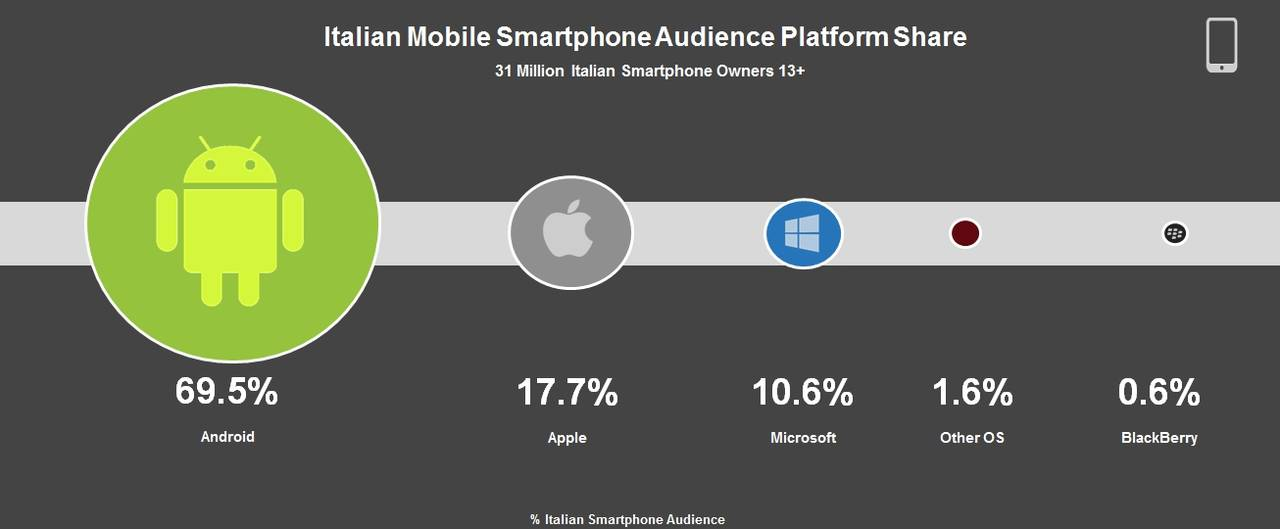
\includegraphics[width=\columnwidth]{tecnologie/mercato} 
    \caption{Frammentazione SO del mercato italiano nel 2016}
\end{figure}

Compresa la necessità di sviluppare più versioni della medesima applicazione in diverse piattaforme, il problema si sposta sulle risorse economiche e sul tempo che si ha a disposizione per lo sviluppo. Infatti lo sviluppo in differenti piattaforme comporta l'utilizzo di differenti linguaggi di programmazione e quindi la necessità di più programmatori esperti, precisamente almeno uno per piattaforma. Altre variabili di cui tener conto sono gli strumenti di sviluppo necessari, le \textit{API} che si hanno a disposizione e fattori quali i sensori disponibili sui dispositivi, la dimensione degli schermi e le capacità di calcolo differenti.

L'obiettivo che i \textit{framework cross-platform} cercano di raggiungere è la risoluzione di tutti questi problemi in maniera efficiente ed efficace in termini di risorse utilizzate, quindi, più precisamente, di ridurre gli effetti negativi della frammentazione del mercato.

\begin{figure}[!h] 
    \centering 
    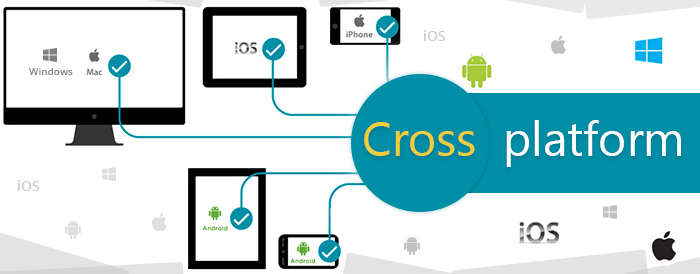
\includegraphics[width=\columnwidth]{tecnologie/framework} 
    \caption{L'obiettivo dei \textit{framework cross-platform}}
\end{figure}

Per raggiungere questo obiettivo i \textit{framework cross-platform} permettono l'utilizzo di un solo linguaggio di programmazione, o di un insieme ristretto di linguaggi, per lo sviluppo di un unico codice sorgente che viene poi in secondo luogo convertito nel codice nativo delle piattaforme sulle quali si desidera distribuire l'applicazione. 

Per concludere, dati oggettivi dimostrano che durante il 2016 l'utilizzo dei \textit{framework cross-platform} ha portato ad un risparmio in termini di risorse economiche nell'80\% dei casi e ad un risparmio di tempo nell'83\% dei casi.

\subsection{Approcci alla base dei framework cross-platform}

Per la scelta del \textit{framework cross-platform} più idoneo al problema è stato richiesto di studiare gli approcci secondo i quali i framework permettono la distribuzione su varie piattaforme. Esistono principalmente quattro approcci in base ai quali i \textit{framework} possono essere classificati:
\begin{itemize}
	\item approccio web;
	\item approccio ibrido;
	\item approccio interpretato;
	\item approccio \textit{cross-compiled}.
\end{itemize}

In questa tesi vengono presentati solamente l'approccio ibrido e quello interpretato, poiché utilizzati dai \textit{framework} proposti dal \textit{tutor} aziendale.

L'approccio ibrido si interpone tra la realizzazione di un'applicazione web e lo sviluppo di un'applicazione mobile in codice nativo. In questo tipo di approccio l'applicazione viene sviluppata utilizzando tecnologie web ed eseguita all'interno di un container nativo sul dispositivo mobile. Per eseguire l'applicazione viene utilizzato il motore di \textit{rendering} del browser del dispositivo mobile che si occupa di interpretare e visualizzare il contenuto \textit{HTML} dell'applicazione tramite una visualizzazione web a schermo intero. L'accesso alle funzionalità native offerte dal dispositivo mobile è permesso grazie ad un livello astratto che si interpone tra l'applicazione ibrida e tali funzionalità. Questo livello astratto espone le funzionalità tramite \textit{API} \textit{Javascript}. 

\begin{figure}[!h] 
    \centering 
    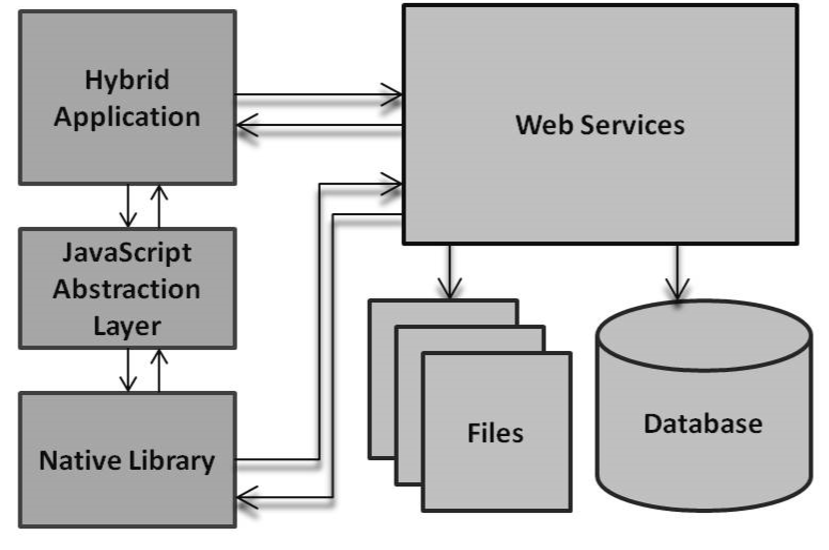
\includegraphics[width=0.9\columnwidth]{tecnologie/ibrido} 
    \caption{Architettura di un'applicazione ibrida}
\end{figure}

Nel caso delle applicazioni interpretate il codice sorgente dell'applicazione viene distribuito sul dispositivo mobile e in seguito interpretato da un interprete che si occupa di eseguire il codice a \textit{run-time}. Anche in questo caso le funzionalità native vengono rese disponibili da un livello astratto. La caratteristica principale dell'interprete è che eseguendo il codice sorgente su differenti piattaforme, esso supporta lo sviluppo \textit{cross-platform} delle applicazioni. L'applicazione interpretata interagisce con il livello astratto per accedere alle \textit{API} native. Uno dei vantaggi dell'approccio interpretato è che utilizza elementi delle specifiche interfacce utente native per l'interazione utente. Infine, la logica applicativa è catturata in maniera del tutto indipendente dalla piattaforma sulla quale l'applicazione viene eseguita.

\begin{figure}[!h] 
    \centering 
    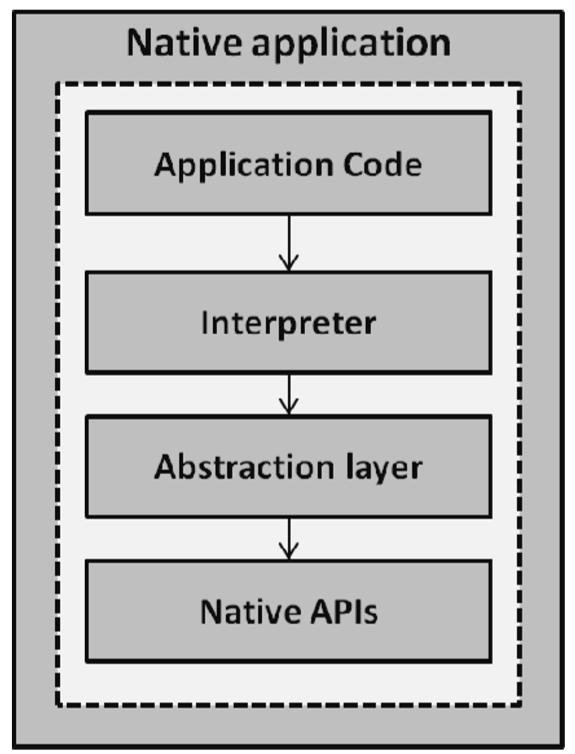
\includegraphics[height=8cm,width=0.6\columnwidth]{tecnologie/interpretato} 
    \caption{Architettura di un'applicazione interpretata}
\end{figure}

\newpage

\subsection{Xamarin}

Si tratta di un \textit{framework cross-platform} di proprietà dell'azienda \textit{Microsoft} che utilizza due approcci differenti, l'approccio interpretato per l'ambiente \textit{Android} e \textit{Windows}, e l'approccio compilato per l'ambiente \textit{iOS}. Più precisamente, per le piattaforme \textit{Android} e \textit{Windows} è possibile generare l'applicazione direttamente tramite i \textit{tool} messi a disposizione dal \textit{framework} e successivamente distribuirla sui rispettivi \textit{store}, mentre per la piattaforma \textit{iOS} è necessario un passo aggiuntivo. È richiesto, infatti, il passaggio per una macchina \textit{Apple} che abbia installato \textit{XCode} per eseguire la compilazione dell'applicazione. Infine, \textit{Xamarin} richiede che venga utilizzato il linguaggio \textit{C\#} per lo sviluppo dell'applicazione. Nella figura sottostante viene presentata l'architettura di \textit{Xamarin}.

\begin{figure}[!h] 
    \centering 
    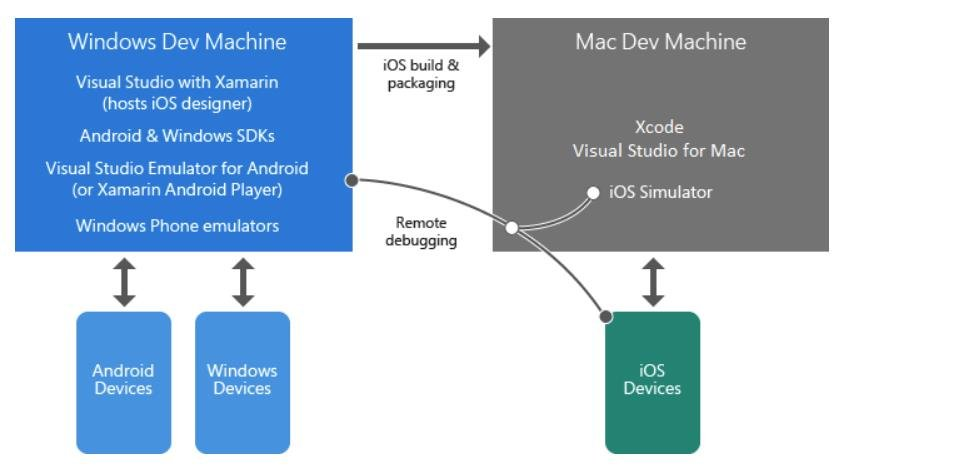
\includegraphics[width=\columnwidth]{tecnologie/xamarinArchitecture} 
    \caption{Architettura del \textit{framework Xamarin}}
\end{figure}

\subsection{PhoneGap}

Si tratta di un \textit{framework cross-platform} di proprietà dell'azienda \textit{Apache} che utilizza un approccio di tipo ibrido. Quindi permette la realizzazione di applicazioni mobile tramite l'utilizzo di tecnologie web, che sono al giorno d'oggi strumenti conosciuti da tutti gli sviluppatori. L'accesso ai componenti hardware dei dispositivi mobile è permesso grazie all'utilizzo di \textit{plugin} scaricabili dalla pagina ufficiale del \textit{framework}. Vantaggi importanti del \textit{framework} sono la presenza di documentazione completa per i \textit{plugin} e la presenza di una \textit{community} grande e sempre disponibile. Infine \textit{PhoneGap} rende disponibili degli strumenti che facilitano lo sviluppo dell'applicazione: \textit{PhoneGap Desktop App}, \textit{PhoneGap CLI}, \textit{PhoneGap App} e \textit{PhoneGap Build}. I primi tre strumenti fanno parte dell'ambiente di sviluppo utilizzato durante lo \textit{stage} e verranno descritti successivamente. \textit{PhoneGap Build} è uno strumento che permette la build dell'applicazione direttamente su un \textit{server} \textit{cloud Adobe} a partire da un file zip contenente la cartella con il codice sorgente dell'applicazione. In seguito alla \textit{build} è possibile generare e scaricare automaticamente l'applicazione per \textit{Windows} o per \textit{Android}. Per quanto riguarda \textit{iOS}, è necessario fornire i certificati richiesti da \textit{Apple} per la distribuzione dell'applicazione. Nella pagina successiva vengono presentate l'architettura di \textit{PhoneGap} e una figura illustrativa di \textit{PhoneGap Build}.

\begin{figure}[!h] 
    \centering 
    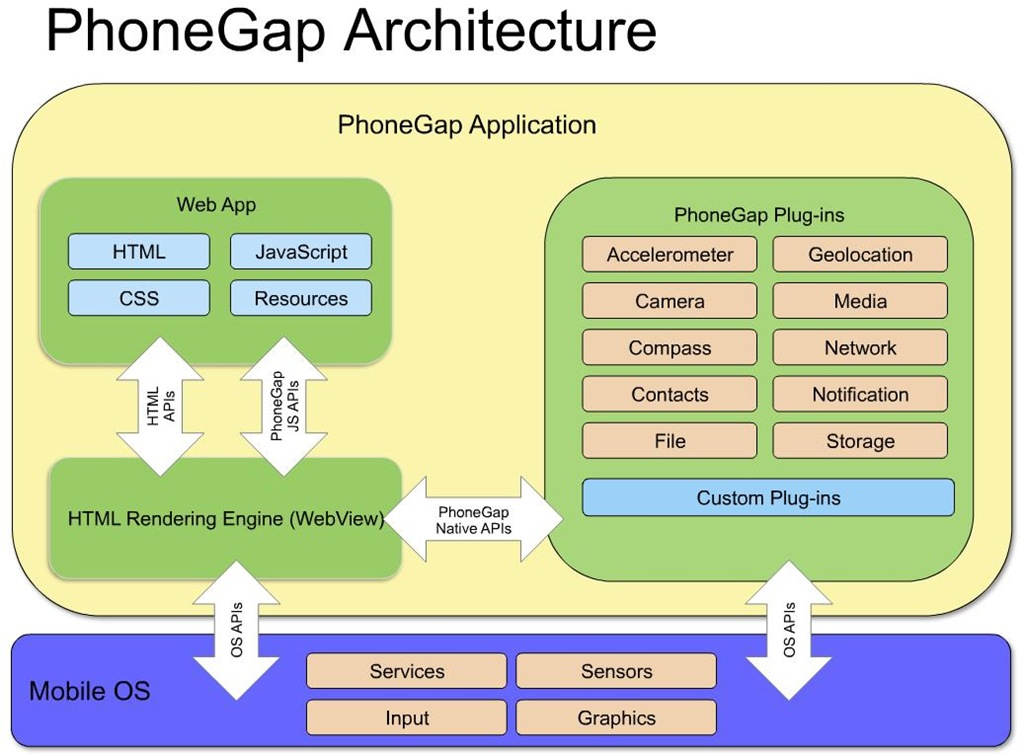
\includegraphics[width=0.9\columnwidth]{tecnologie/phonegapArchitecture} 
    \caption{Architettura del \textit{framework PhoneGap}}
\end{figure}

\begin{figure}[!h] 
    \centering 
    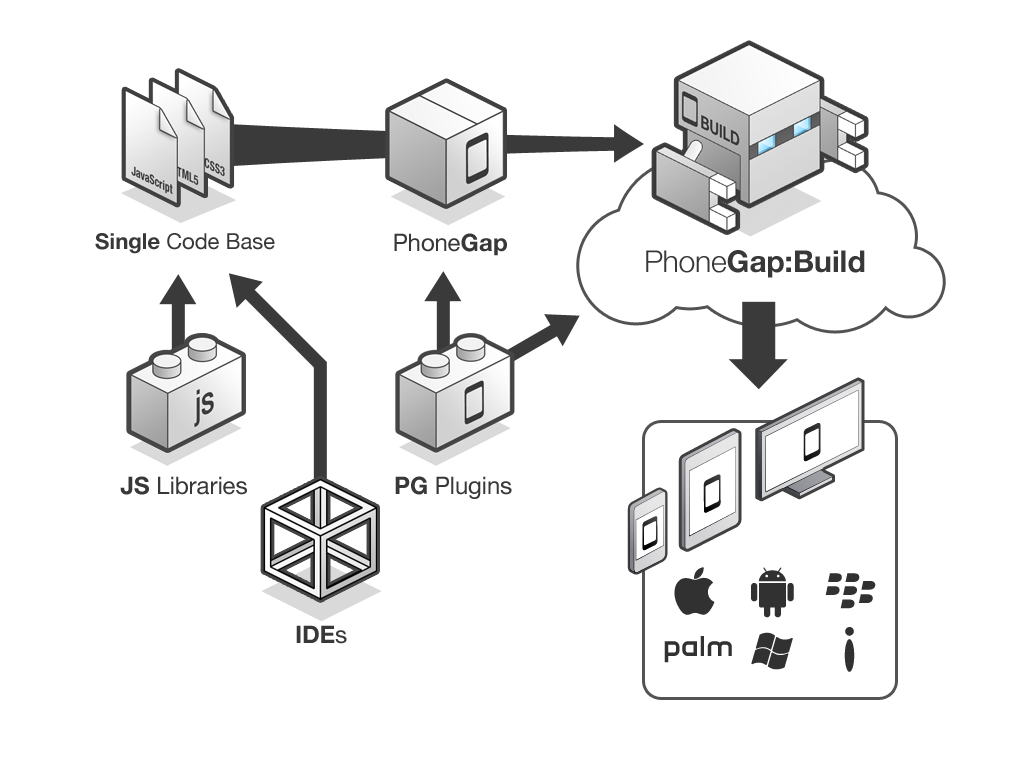
\includegraphics[width=\columnwidth]{tecnologie/phonegapBuild} 
    \caption{Figura illustrativa di \textit{PhoneGap Build}}
\end{figure}

\newpage


\subsection{La scelta di PhoneGap}

Lo stagista ha optato per il \textit{framework PhoneGap} per tre motivi sostanziali:
\begin{enumerate}
	\item \textbf{linguaggio di programmazione}: \textit{PhoneGap} richiedeva l'utilizzo di tecnologie web, già conosciute e apprese dallo stagista all'Università. Lo studio del linguaggio \textit{C\#}, utilizzato da \textit{Xamarin}, avrebbe richiesto un periodo di formazione che avrebbe sforato le 40 ore messe a disposizione per la formazione sulle tecnologie;
	\item \textbf{linguaggio \textit{Javascript}}: come detto precedentemente, lo stagista era interessato ad approfondire il linguaggio \textit{Javascript}, richiesto al giorno d'oggi dalla maggior parte delle aziende che si occupano della realizzazione di applicazioni web;
	\item \textbf{facilità nello sviluppo dell'interfaccia grafica}: utilizzando tecnologie web risultava semplice progettare e sviluppare un'interfaccia grafica \glossaryItem{responsive}, e quindi in grado di adattarsi alla maggior parte dei dispositivi mobile presenti sul mercato.
\end{enumerate}

\section{Ambiente di sviluppo}

Durante il periodo di \textit{stage} è stato utilizzato uno specifico ambiente di lavoro, comprendente tecnologie in parte imposte dal \textit{tutor} aziendale e in parte scelte dallo stagista. La qualità di queste tecnologie ha impatto diretto sulla qualità di processo e quindi sulla qualità di prodotto, per cui è importante tenere l'ambiente di lavoro costantemente completo, ordinato e aggiornato. Per ottenere questo, lo stagista ha dovuto analizzare le tecnologie scelte per assicurarsi che fossero le più adatte per il dominio del problema.

\subsection{Suite di PhoneGap}

La suite di \textit{PhoneGap} ha costituito parte fondamentale dell'ambiente di lavoro. Sono stati utilizzati i seguenti software della suite:
\begin{itemize}
	\item \textbf{\textit{PhoneGap Desktop App}}: utilizzata inizialmente per prendere dimestichezza con il \textit{framework};
	\item \textbf{\textit{PhoneGap CLI}}: utilizzata dopo aver preso dimestichezza con il \textit{framework};
	\item \textbf{\textit{PhoneGap App}}: utilizzata inizialmente per testare l'applicazione generata dal \textit{framework}.
\end{itemize}

\textit{PhoneGap Desktop App} è un'applicazione installabile su \textit{Windows} o \textit{Mac} con la quale è possibile iniziare ad utilizzare il \textit{framework} con estrema facilità. Essa fornisce un'interfaccia grafica per la creazione, la gestione e il \textit{testing} di progetti \textit{PhoneGap}. Per testare l'applicazione è sufficiente essere in possesso di un dispositivo \textit{Android} con installata l'applicazione \textit{PhoneGap App}. L'applicazione in versione \textit{iOS} è stata rimossa dall'\textit{App Store} per non aver passato i controlli di qualità \textit{Apple}. Nella pagina successiva viene presentata una figura che mostra l'interfaccia grafica di \textit{PhoneGap Desktop App}.

\begin{figure}[!h] 
    \centering 
    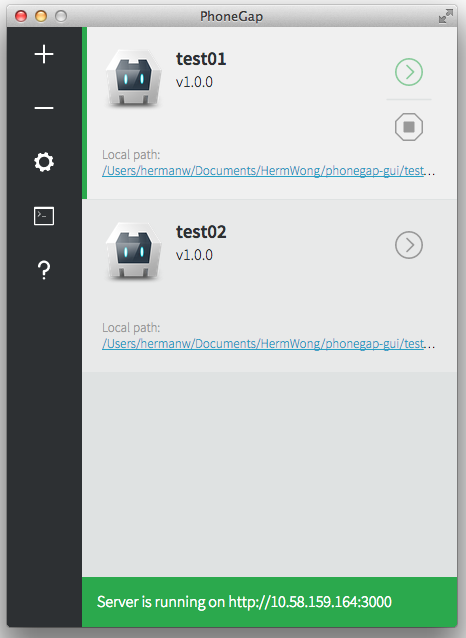
\includegraphics[width=0.8\columnwidth]{tecnologie/phonegapDesktop} 
    \caption{\textit{PhoneGap Desktop App}}
\end{figure}

\newpage

\textit{PhoneGap CLI} estende le funzionalità offerte da \textit{PhoneGap Desktop App} tramite un'interfaccia a riga di comando. Tale applicazione era lo strumento principale per l'utilizzo di \textit{PhoneGap} prima della creazione dell'app desktop. \textit{PhoneGap CLI} può essere utilizzata singolarmente o assieme a \textit{PhoneGap Desktop App} e/o \textit{PhoneGap Build}.

\textit{PhoneGap App} è un'applicazione mobile, installabile solamente su dispositivi \textit{Android}, con la quale è possibile testare l'applicazione \textit{PhoneGap} senza generare ed installare nessun file applicazione. Per testare l'applicazione è sufficiente avviare l'esecuzione del progetto su \textit{PhoneGap Desktop App} e collegare il computer di sviluppo e il dispositivo su cui è installata \textit{PhoneGap App} alla stessa rete \textit{Wi-Fi}. Dopo aver completato questi semplici passaggi, viene richiesto di inserire su \textit{PhoneGap App} l'indirizzo di rete su cui il progetto è stato messo in esecuzione da \textit{PhoneGap Desktop App}. Dopo aver inserito questo indirizzo, la reale applicazione verrà visualizzata sullo \textit{smartphone} e sarà possibile testarla completamente.

\begin{figure}[!h] 
    \centering 
    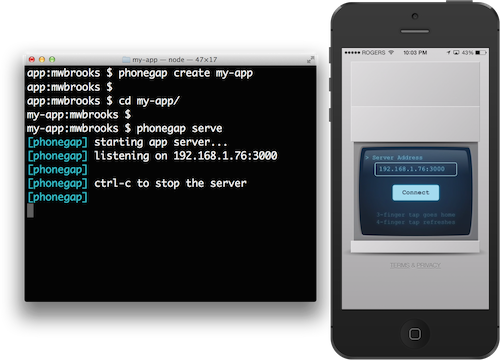
\includegraphics[width=0.8\columnwidth]{tecnologie/phonegapCLIApp} 
    \caption{\textit{PhoneGap CLI} e \textit{PhoneGap App}}
\end{figure}

\subsection{Editor e IDE}

\subsubsection{Sublime Text 3.0}

Per lo sviluppo del progetto \textit{PhoneGap} è stato utilizzato l'editor \textit{Sublime Text 3.0}, ritenuto dallo stagista il più semplice e leggero per la realizzazione di applicazioni web. 

\begin{figure}[!h] 
    \centering 
    
\includegraphics[height=4cm,width=4cm]{tecnologie/sublime} 
    \caption{Logo di \textit{Sublime Text 3.0}}
\end{figure}

\subsubsection{Android Studio}

Durante lo \textit{stage}, l'applicazione \textit{Android} generata tramite i \textit{tool} offerti dal \textit{framework PhoneGap} non era soddisfacente: spesso non funzionava o l'interfaccia grafica non rispecchiava quella desiderata. Per cui è stato necessario installare \textit{Android Studio} per applicare gli accorgimenti in codice nativo necessari a rendere l'app usabile. \textit{Android Studio} è un ambiente di sviluppo integrato (\textit{IDE}) basato sul software di \textit{JetBrains IntelliJ IDEA} e progettato specificamente per lo sviluppo di applicazioni \textit{Android}.

\begin{figure}[!h] 
    \centering 
    
\includegraphics[height=4.5cm,width=4.5cm]{tecnologie/androidStudio} 
    \caption{Logo di \textit{Android Studio}}
\end{figure}

\subsubsection{XCode}

Durante lo \textit{stage}, l'applicazione iOS generata tramite i \textit{tool} offerti dal \textit{framework PhoneGap} non era soddisfacente: spesso non funzionava o l'interfaccia grafica non rispecchiava quella desiderata. Per cui è stato necessario installare \textit{XCode} per applicare gli accorgimenti in codice nativo necessari a rendere l'app usabile. \textit{Xcode} è un ambiente di sviluppo integrato (\textit{IDE}) contenente una suite di strumenti utili allo sviluppo di software per i sistemi \textit{macOS}, \textit{iOS}, \textit{watchOS} e \textit{tvOS}. È completamente sviluppato e mantenuto da \textit{Apple}.

\begin{figure}[!h] 
    \centering 
    
\includegraphics[height=4cm,width=5cm]{tecnologie/xCode} 
    \caption{Logo di \textit{XCode}}
\end{figure}

\subsubsection{Eclipse JEE}

Durante lo \textit{stage} è stata richiesta la realizzazione di un servizio web che si interponesse tra la logica applicativa di \textit{moviORDER} e il \textit{database} presente sul \textit{server Azure} di \visione{}. Il servizio web è stato realizzato in linguaggio \textit{Java} tramite l'utilizzo di oggetti \textit{servlet}. Per la realizzazione degli oggetti \textit{servlet} è stato utilizzato l'\textit{IDE Eclipse JEE} che offre buoni strumenti per lo sviluppo di applicazioni web \textit{Java}. \textit{Eclipse} è un ambiente di sviluppo integrato multi-linguaggio e multipiattaforma, ideato da un consorzio di grandi società quali \textit{Ericsson}, \textit{HP}, \textit{IBM}, \textit{Intel}, \textit{MontaVista Software}, \textit{QNX}, \textit{SAP} e \textit{Serena Software}, chiamato \textit{Eclipse Foundation}.

\begin{figure}[!h] 
    \centering 
    
\includegraphics[width=0.8\columnwidth]{tecnologie/eclipse} 
    \caption{Logo di \textit{Eclipse}}
\end{figure}

\subsection{Gestione DBMS}

Durante il progetto, per la gestione del \textit{database} di \textit{moviORDER} è stato utilizzato il \glossaryItem{DBMS} \textit{Microsoft SQL Server}. Per una gestione veloce ed ottimale dello stesso si è deciso di usare il software \textit{SQL Server Management Studio}. \textit{SQL Server Management Studio} (\textit{SSMS}) è un'applicazione software usata per configurare, gestire e amministrare \textit{database}, in locale o su un \textit{server} \textit{cloud}, con il \textit{DBMS Microsoft SQL Server}. 

\begin{figure}[!h] 
    \centering 
    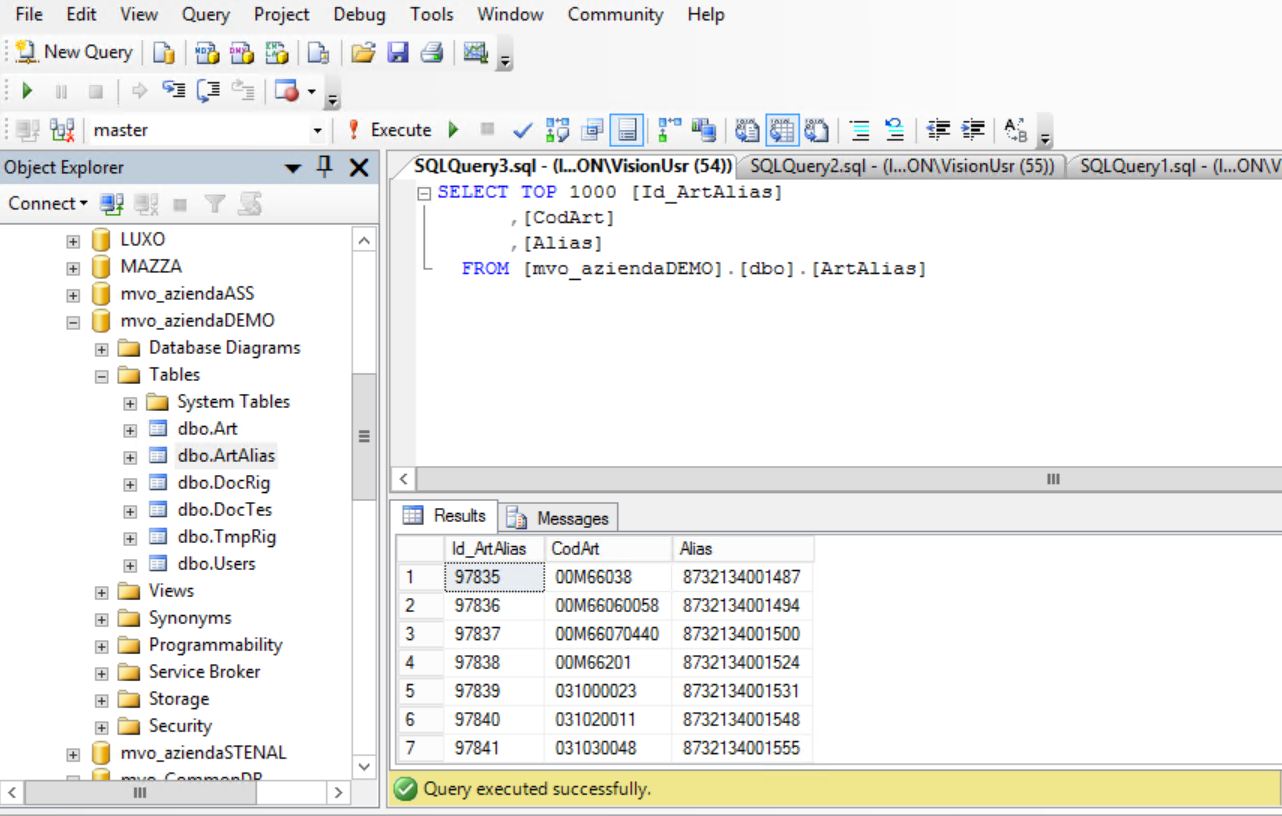
\includegraphics[width=\columnwidth]{tecnologie/ssms} 
    \caption{\textit{Screenshot} di \textit{SQL Server Management Studio}}
\end{figure}

\newpage

\subsection{Server web}

Per lo sviluppo del progetto è stato realizzato un servizio web che fornisce una \textit{API} all'applicazione per poter accedere ai dati contenuti nel \textit{database} sul \textit{server} \textit{cloud} di \visione{}. Per permettere l'esecuzione del servizio web sul \textit{server} \textit{cloud} si è utilizzato \textit{Apache Tomcat}. \textit{Apache Tomcat} (o semplicemente \textit{Tomcat}) è un web \textit{server} (nella forma di contenitore \textit{servlet}) \textit{open source} sviluppato dalla \textit{Apache Software Foundation}. Implementa le specifiche \textit{JavaServer Pages} (\textit{JSP}) e \textit{servlet}, fornendo quindi una piattaforma software per l'esecuzione di applicazioni Web sviluppate in linguaggio \textit{Java}.

\begin{figure}[!h] 
    \centering 
    
\includegraphics[height=4cm,width=5cm]{tecnologie/tomcat} 
    \caption{Logo di \textit{Apache Tomcat}}
\end{figure}

\subsection{Cloud computing}

Il servizio web e il \textit{database} con il quale l'applicazione interagisce per offrire le funzionalità all'utente risiedono su un \textit{server} cloud di \visione{}. Tale \textit{server} è di proprietà di \textit{Microsoft Azure}. \textit{Microsoft Azure} (precedentemente nota come \textit{Windows Azure}) è la piattaforma \textit{cloud} pubblica di \textit{Microsoft}, che offre servizi di \textit{cloud computing}. Tramite Azure vengono erogati servizi appartenenti a diverse categorie quali: risorse di elaborazione, archiviazione e memorizzazione dati, trasmissione dati e interconnessione di reti, analisi, \textit{intelligence}, apprendimento automatico, sicurezza e gestione delle identità, monitoraggio e gestione, nonché servizi per lo sviluppo di applicazioni. Per accedere al \textit{server} da remoto è stato utilizzato il software Connessione Desktop Remoto di \textit{Windows}.

\begin{figure}[!h] 
    \centering 
    
\includegraphics[width=0.8\columnwidth]{tecnologie/azure} 
    \caption{Logo di \textit{Microsoft Azure}}
\end{figure}

\subsection{Strumenti di testing}

Durante lo sviluppo di \textit{moviORDER} sono stati eseguiti dei test per verificare il corretto funzionamento del servizio web e dell'applicazione. Per il test delle \textit{API} del servizio web si è utilizzato \textit{Postman}. \textit{Postman} è uno strumento di \textit{API testing} che permette di testare \textit{API} direttamente, o come parte di test d'integrazione, per determinare se soddisfano criteri di funzionalità, affidabilità, performance e sicurezza. Nel caso di \textit{moviORDER}, il test avviene tramite l'invio di una richiesta \textit{HTTP POST}, con parametri impostabili, alla \textit{API} sul \textit{server} \textit{cloud}. In seguito alla richiesta il software visualizza il \textit{JSON} restituito dalla \textit{API} e lo sviluppatore può verificare se la risposta del servizio è quella attesa.

\begin{figure}[!h] 
    \centering 
    
\includegraphics[height=4cm,width=5cm]{tecnologie/postman} 
    \caption{Logo di \textit{Postman}}
\end{figure}

Per testare il corretto funzionamento dell'applicazione si è utilizzata la console del browser \textit{Google Chrome} facente parte degli strumenti offerti dallo stesso per gli sviluppatori web. Tramite la console è stato possibile verificare la logica applicativa di \textit{moviORDER}, poiché scritta in \textit{JavaScript}.

\begin{figure}[!h] 
    \centering 
    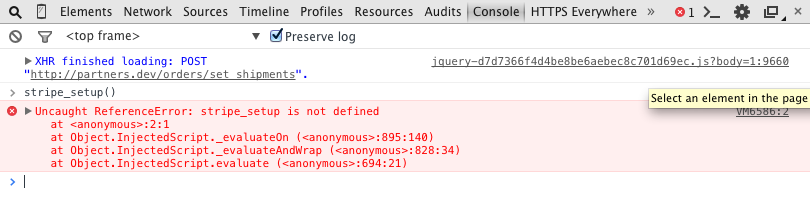
\includegraphics[width=\columnwidth]{tecnologie/console} 
    \caption{\textit{Screenshot} della console di \textit{Google Chrome}}
\end{figure}

\newpage

\subsection{Strumenti di versioning e ticketing}

Per scelta dello stagista il progetto è stato sottoposto a controllo di versione in ogni sua parte: applicazione, servizio web e documentazione. Questo ha permesso, principalmente nel caso dell'applicazione, di tornare a \glossaryItem{baseline} sicure nel caso di sovrascritture o perdite accidentali, o \textit{commit} di codice con errori di programmazione. Per il controllo di versione si è utilizzato lo strumento \textit{Git} e in particolare il servizio di hosting \textit{GitHub}. Lo stagista ha scelto tali software perché già utilizzati in progetti didattici durante l'Università.

\begin{figure}[!h] 
    \centering 
    
\includegraphics[height=5cm,width=5cm]{tecnologie/git} 
    \caption{Logo di \textit{GitHub}}
\end{figure}

Lo stagista ha scelto inoltre di utilizzare uno strumento di \textit{ticketing} per facilitare la pianificazione del progetto. Lo strumento scelto è \textit{Asana}. \textit{Asana} è un'applicazione web e mobile progettata per aiutare i team ad organizzare, tracciare e gestire il loro lavoro. In particolare, lo strumento è stato utilizzato per dare una scadenza ai ticket in base alla pianificazione decisa insieme al \textit{tutor} aziendale all'inizio del periodo di \textit{stage}.

\begin{figure}[!h] 
    \centering 
    
\includegraphics[height=5cm,width=7cm]{tecnologie/asana} 
    \caption{Logo di \textit{Asana}}
\end{figure}

\subsection{Strumenti di modellazione e documentazione}

Il progetto ha richiesto lo sviluppo di diagrammi di \textit{Gantt} in fase di pianificazione e di diagrammi \textit{UML} in fase di analisi dei requisiti e di progettazione. Per la realizzazione dei diagrammi di \textit{Gantt} si è utilizzato il software \textit{Gantt Project}, per i diagrammi \textit{UML} dei casi d'uso si è utilizzato il software \textit{Astah UML}, mentre per i diagrammi \textit{UML} dei \textit{package} e delle classi si è utilizzato il software \textit{Visual Paradigm CE}. I software sono stati scelti perché già appresi durante il progetto di Ingegneria del Software all'Università.

\begin{figure}[!h] 
    \centering 
    	\subfloat{
\includegraphics[width=0.33\columnwidth]{tecnologie/gantt}}
    	\subfloat{
\includegraphics[width=0.33\columnwidth]{tecnologie/astah}} 
    	\subfloat{
\includegraphics[width=0.33\columnwidth]{tecnologie/vp}} 
    \caption{Loghi di \textit{Gantt Project}, \textit{Astah UML} e \textit{Visual Paradigm CE}}
\end{figure}

Per la realizzazione dei diagrammi \textit{ER} e delle figure illustrative dell'architettura del prodotto si è utilizzato il software \textit{Lucidchart}. Per la stesura della documentazione si è utilizzato l'editor \textit{TexMaker}, anch'esso utilizzato durante il progetto di Ingegneria del Software. \textit{TexMaker} permette l'inserimento veloce dei comandi \LaTeX{} più utilizzati tramite la pressione di pulsanti sull'interfaccia grafica, l'integrazione con un dizionario per il controllo ortografico e la compilazione e visione del pdf prodotto.

\begin{figure}[!h] 
    \centering 
    \subfloat{
\includegraphics[height=4.5cm,width=4.5cm]{tecnologie/lucid}}
    \subfloat{
\includegraphics[height=4.5cm,width=4.5cm]{tecnologie/tex}}
    \caption{Loghi di \textit{Lucidchart} e \textit{TexMaker}}
\end{figure}

\subsection{Linguaggi di programmazione e murkup}

\subsubsection{HTML5, CSS3 e JavaScript}

Lo stagista ha dovuto utilizzare i linguaggi \textit{HTML5}, \textit{CSS3} e \textit{JavaScript} in quanto ha scelto il \textit{framework cross-platform PhoneGap}, il quale richiede l'utilizzo di tecnologie web per lo sviluppo dell'applicazione mobile. In particolare, \textit{HTML5} è stato scelto perché include un insieme di funzionalità che permettono di valorizzare le interfacce mobile. Alcune di queste evidenziano come \textit{HTML5} sia già per sua natura orientato al mobile. In particolare \textit{HTML5} fornisce \textit{API} per:
\begin{itemize}
	\item \textbf{geolocalizzazione}: con la scrittura di poco codice, forniscono la posizione del dispositivo in coordinate terrestri. Quindi, la stessa funzionalità su uno \textit{smartphone} o un \textit{tablet} fornisce la posizione dell'utente stesso;
	\item \textbf{eventi \textit{touch}}: mentre i meccanismi di input nei PC consistono per lo più nella tastiera e nel mouse, nei dispositivi mobili quasi tutto passa per il \textit{touch screen}, e avere funzionalità comode per gestire questo strumento consente un'interazione più ricca e senza limitazioni per l'utente. Le gestualità da attuare su un display, nel mondo mobile, costituiscono un vero e proprio linguaggio fondamentale nella \textit{user experience};
	\item \textbf{controllo batteria}: considerata l'importanza rivestita dalle risorse energetiche, l'esistenza stessa di questa libreria nel linguaggio dimostra come il suo impiego sia particolarmente mirato al panorama mobile.
\end{itemize}

Ciò che ha favorito la scelta di \textit{CSS3} sono le \glossaryItem{media queries}. Esse permettono di definire regole stilistiche in base alla tipologia del mezzo di visualizzazione, delle sue dimensioni nonchè della sua attuale disposizione (\textit{portrait} o \textit{landscape}). Ciò influisce non solo sull'aspetto esteriore degli elementi ma anche sul loro posizionamento e quindi sulla struttura stessa dell'interfaccia.

Per quanto riguarda il linguaggio \textit{JavaScript} è stato utilizzato \textit{JavaScript} puro senza l'utilizzo di \textit{framework} o \glossaryItem{JQuery}. Una particolarità del linguaggio, detta \textit{AJAX}, ha reso possibile eseguire chiamate alla \textit{API} del servizio web di \textit{moviORDER} e modificare la pagina \textit{HTML} di conseguenza in base alla risposta. \textit{AJAX}, acronimo di \textit{Asynchronous JavaScript and XML}, è una tecnica di sviluppo software per la realizzazione di applicazioni web interattive (\textit{Rich Internet Application}). Lo sviluppo di applicazioni \textit{HTML} con \textit{AJAX} si basa su uno scambio di dati in background fra web browser e \textit{server}, che consente l'aggiornamento dinamico di una pagina web senza esplicito ricaricamento da parte dell'utente.

\begin{figure}[!h] 
    \centering 
    	
\includegraphics[width=0.8\columnwidth]{tecnologie/html5}
    \caption{Loghi di \textit{HTML5}, \textit{CSS3} e \textit{JavaScript}}
\end{figure}

I linguaggi scelti, grazie alle loro caratteristiche che li rendono orientati al mobile, insieme ai meccanismi che il \textit{framework PhoneGap} utilizza per convertire la \textit{web application} in applicazione mobile, permettono di dover effettuare meno modifiche in seguito per perfezionare l'applicazione su \textit{Android} e \textit{iOS}.

\subsubsection{Java}

Per la realizzazione del servizio web che permette all'applicazione di interfacciarsi con il \textit{database} sul \textit{server} \textit{cloud} di \visione{} si è utilizzato il linguaggio \textit{Java}. La scelta è stata fatta dallo stagista tra due alternative in cui rientrava anche \textit{PHP}. È stato scelto Java in quanto possiede un compilatore, è più facilmente \textit{debbugabile} rispetto a \textit{PHP} e permette l'utilizzo di oggetti \textit{servlet}.  I \textit{servlet} sono oggetti scritti in linguaggio \textit{Java} che operano all'interno di un \textit{server web} (nel caso del progetto Tomcat) oppure un \textit{server} per applicazioni permettendo la creazione di applicazione web. Nel caso del progetto, i \textit{servlet} hanno premesso lo sviluppo della \textit{API} che costituisce il servizio web. Una descrizione della \textit{API}, di come i \textit{servlet} sono stati utilizzati nel progetto e di come la \textit{API} viene interrogata dall'applicazione è presente in sezione §\ref{api}.

\begin{figure}[!h] 
    \centering 
    
\includegraphics[height=4.5cm,width=4.5cm]{tecnologie/java} 
    \caption{Logo di \textit{Java}}
\end{figure}

\subsubsection{\LaTeX{}}

Per lo sviluppo della documentazione annessa a \textit{moviORDER} è stato utilizzato il linguaggio \LaTeX{}. La scelta è ricaduta su \LaTeX{} perché già appreso e utilizzato durante il progetto di Ingegneria del Software. \LaTeX{} è un linguaggio di \textit{markup} usato per la preparazione di testi basato sul programma di composizione tipografica TEX. Fornisce funzioni di \textit{desktop publishing} programmabili e mezzi per l'automazione della maggior parte della composizione tipografica, inclusa la numerazione, i riferimenti incrociati, tabelle e figure, organizzazione delle pagine, bibliografie e molto altro. Infine la particolarità più utile del linguaggio è l'esistenza di \textit{community} che rendono disponibili \glossaryItem{template} riutilizzabili come quello che è stato utilizzato per la stesura di questa tesi.

\begin{figure}[!h] 
    \centering 
    
\includegraphics[height=3cm,width=6cm]{tecnologie/latex} 
    \caption{Logo di \LaTeX{}}
\end{figure}

\subsection{DBMS}

Per la creazione, gestione e amministrazione di \textit{database} è stato utilizzato il \textit{DBMS Microsoft SQL Server}. È stato scelto questo software perché già ampiamente utilizzato all'interno dell'azienda. Questo permetterà agli sviluppatori di \visione{} di lavorare sul \textit{database} di \textit{moviORDER} con un linguaggio già pienamente conosciuto. \textit{Microsoft SQL Server} usa una variante del linguaggio \textit{SQL} standard chiamata \textit{Transact-SQL} (\textit{T-SQL}). \textit{Transact-SQL} espande le prestazioni di \textit{SQL} aggiungendo:
\begin{itemize}
	\item funzioni per controllo di flusso;
	\item possibilità di definire variabili locali;
	\item varie funzioni per la manipolazione di stringhe, date ed espressioni matematiche;
	\item miglioramento delle istruzioni \textit{DELETE} e \textit{UPDATE}.
\end{itemize}

\begin{figure}[!h] 
    \centering 
    
\includegraphics[height=5cm,width=7cm]{tecnologie/sqlserver} 
    \caption{Logo di \textit{SQL Server}}
\end{figure}